% ======================= Pre-Amble =========================
      
%Format
\documentclass[11pt, oneside]{article}   	% use "amsart" instead of "article" for AMSLaTeX format 
                     						%imports package {article} and specify option(s) [11pt, oneside]
\usepackage{geometry}                		% See geometry.pdf to learn the layout options. There are lots. 
    \geometry{letterpaper}                   		% ... or a4paper or a5paper or ... 
    %\geometry{landscape}                		% Activate for rotated page geometry

\usepackage[parfill]{parskip}    		        % Activate to begin paragraphs with an empty line rather than an indent

    %Colours
    \usepackage{graphicx, subcaption}
    \usepackage[usenames, dvipsnames]{color}     % font colour:    \textcolor{<colour>}{text}
          									%highlight text:  \colorbox{<color>}{text}
    \usepackage{soul}						%highlight text: \hl{}     %only  yellow								
    									%list of colours: https://www.sharelatex.com/learn/Using_colours_in_LaTeX
    									
    %Bullets
    \usepackage{enumerate}     %specify type of enumeration: \being{enumerate}[<type of enumeration>]
    
    %Footnote Spacing
    \setlength{\footnotesep}{0.4cm}                  %specify spacing b/w footnotes
    \setlength{\skip\footins}{0.6cm}                    % space b/w footnotes and textbody


%Mattematics
    %American Mathematics Society packages
    \usepackage{amsmath}	   %math
    \usepackage{amssymb}       %symbols
    \usepackage{amsthm}          %theorems
    \newtheorem{proposition}{Proposition}

    %QED
    \newcommand*{\QEDA}{\hfill\ensuremath{\blacksquare}}         %make qed filled square:    \QEDA
    \newcommand*{\QEDB}{\hfill\ensuremath{\square}}               %make qed empty square: \QEDB 
    
    \renewcommand\qedsymbol{\ensuremath{\blacksquare}}		%Proof environment


%Figures
\usepackage{caption}
\captionsetup[figure]{labelfont=bf}    %make figure labels boldface
\captionsetup[table]{labelfont=bf}     %make table labels boldface

\usepackage[hidelinks]{hyperref}                % Allows for clickable references

    %Tables
    \usepackage[none]{hyphenat}                    % Stops breaking-up words in a table (i.e. no hyphens)                                                             
    
    \usepackage{array}   
        \newcolumntype{x}[1]{>{\centering\let\newline\\\arraybackslash\hspace{0pt}}p{#1}}       %center fixed column width: x{<len>}                      
        \newcolumntype{$}{>{\global\let\currentrowstyle\relax}}                                                   % let us apply things (e.g. bold/italicize) to entire row            
        \newcolumntype{^}{>{\currentrowstyle}}
        \newcommand{\rowstyle}[1]{\gdef\currentrowstyle{#1} #1\ignorespaces}
    
    %Images
    \graphicspath{ {images/} }                          %directory that your images are located in within your current directory
    
    %Diagrams
    \usepackage[latin1]{inputenc}
    \usepackage{tikz}
    	\tikzset{line/.style={-latex'}}
        \usepackage{tkz-berge}
        \usetikzlibrary{shapes,arrows}
        \usetikzlibrary{patterns}			%Specify colours of stuff (e.g. vertices): 
        								%	-> set style: \tikzset{VertexStyle/.append style = {minimum size = 8pt, inner sep = 0pt}} 
								%	-> change individual vertices: \AddVertexColor{white}{1,2} 


%Bibliography
\usepackage[numbers,sort&compress]{natbib}   %for multiple references: sorts  (i.e. [1,2] NOT [2, 1] )
                                           				  %                                     compresses (i.e. [1-3] )
\usepackage[nottoc]{tocbibind}                            %add bibliography to table of contents


%Miscellaneous
\usepackage{dirtytalk}    %quotations: use \say  


%================== Header & Footer =========================
\usepackage{fancyhdr}
\usepackage{lastpage}      %ensures you can reference LastPage (i.e. Page 2 of 10)

\renewcommand{\headrulewidth}{0.4pt}		%Decorative Header line: thickness={0.4pt}
\renewcommand{\footrulewidth}{0.4pt}		%Decorative Footer line: thickness={0.4pt}

\setlength{\headheight}{13.6pt} 		%space b/w top of page & header
\setlength{\headsep}{0.3in}		%space b/w page header and body

%Make Header & Footer    
\pagestyle{fancy}
    \lhead{Stephanie Knill} 		% controls the left corner of the header
    \chead{} 					% controls the center of the header
    \rhead{} 					% controls the right corner of the header
    \lfoot{} 					% controls the left corner of the footer
    \cfoot{Page~\thepage\ of \pageref{LastPage}} 				% controls the center of the footer
    												%Page~\thepage\  if just want Page x
    \rfoot{}			 		% controls the right corner of the footer

% =============================== Document ===================================
\begin{document}

% Title Page
\title{MATH 442 --- Assignment 12 \\
\line(1,0){360} \\              %(slope x, y){length of line}
}
\author{
Stephanie Knill \\
54882113 \\
Due: April 6, 2016}

\date{}                   % Activate:  display a given date (e.g. {August 4} ) or no date (empty {} )
                                    %No activate: display current date
\maketitle

%\thispagestyle{empty}                   %Remove header from this (first) page. Change empty -> plain to keep numbering
%								-> Doesn't matter in this case (b/c title page)
%\cleardoublepage


% ================= Questions ================

\section*{Question 67}

\emph{Find a lower bound $>$ 15 and an upper bound $<$ 20 for the Travelling Salesman Problem given by the following graph.}
\begin{figure}[h]                                   
\begin{center}
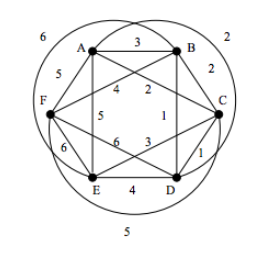
\includegraphics[width=.4\textwidth]{q1.png}
\end{center}
\end{figure}

\cleardoublepage


\section*{Question 68}

\begin{proposition}
A connected digraph $D$ is Eulerian if and only if for each vertex in $D, indeg(v) =outdeg(v).$
\end{proposition}

\begin{proof}
$\Rightarrow$ Assume that a connected digraph $D$ is Eulerian. Let us start at a vertex $v$ and conduct and Euler tour along the edges $e_1, e_2, \ldots, e_n$. As we walk along our tour, whenever we enter a vertex we must also exist it. This will continue until we enter our first vertex $v$ after edge $e_n$. Thus for each vertex, the number of times we have entered (in degree) equals the number of times we have exited (out degree).

$\Leftarrow$ Assume that each vertex in $D$ has $indeg(v)=outdeg(v)$. Let us do an induction on the number of arcs $n$. 

\textbf{Base Case:} $n=2$. Here we have two vertices $i, j$ with edges from $i$ to $j$ and from $j$ to $i$.
\vspace{1cm}

\textbf{Induction Step:} Assume the statement is true for all graphs with $2<n<m$ edges. Since $D$ contains no sinks or sources, we know there exists a closed path $C$. Let us consider the graph
$$G'=G-E(C)$$
This consists of the subgraphs of $G$, each of which contain an Euler tour by the induction assumption. Let us now walk along the edges of $C$, starting at a vertex $u$ until we reach a subgraph. Here, we will trace the Eulerian trail of the subgraph. We will repeat this process until we return to $u$. Thus we now have a closed directed trail containing every edge of $D$, so $D$ is Eulerian and the result follows by induction.
\end{proof}

\section*{Question 69}

\begin{proposition}
If $D$ is an orientation of a simple graph with 10 vertices, then the vertices of $D$ cannot have distinct out degrees.
\end{proposition}

\begin{proof}
Since $D$ is a simple graph, we can have an outdegree at most 9. Thus let us assign outdegrees $0,1,2,3,4,5,6,7,8$, and 9 to our ten vertices, which forms a valid orientation of $D$.
\end{proof}


\section*{Question 70}

\begin{proposition}
Suppose that $G$ is a graph and $D$ is an orientation of $G$ that is strongly connected. If $G$ has a cycle of odd length then $D$ has a directed cycle of odd length.
\end{proposition}

\begin{proof}
Assume that the underlying graph $G$ has a cycle consisting of the vertices $v_1, v_2, \ldots, v_n$ of odd length. Consider each pair of vertices $(v_i, v_{i+1})$. If there exists an arc from $v_i$ to $v_i+1$, we can construct a walk $W_i$ from $v_i$ to $v_{i+1}$ of length 1. If there is an arc from $v_{i+1}$ to $v_i$, then since $D$ is strongly connected, we can find a path $W_i$ from $v_i$ to $v_{i+1}$ of either odd or even length.

\textbf{Case 1:} $W_i$ is of even length. Then we take our even path $W_i$ from $v_i$ to $v_{i+1}$ and add the arc from $v_{i+1}$ to $v_i$ to form a directed cycle of odd length.

\textbf{Case 2:} $W_i$ is of odd length. Then we have some path from $v_i$ to $v_{i+1}$ of odd length, for each $i$. Since we have an odd number of vertices, then if we append each of these walks $W_i$ (i.e. join $v_i$ to $v_{i+1}$ to $v_{i+1}$ to $v_{i+2}, \ldots, v_{i-1}$ to $v_i$), we will have a directed cycle of odd length.
\end{proof}

\section*{Question 71}

\begin{proposition}
If a digraph $D$ contains no cycles, then $D$ contains at least one source and at least one sink.
\end{proposition}

\begin{proof}
Let us conduct induction on the number of vertices $n$.

\textbf{Base Case:} $n=2$
\vspace{1cm}
Here we have 1 source and 1 sink.

\textbf{Induction Step:} Assume the statement holds true for $n=k$ vertices. Let $D$ be a digraph of $n=k+1$ vertices. Now remove a vertex $v$. By the induction assumption, our graph contains at least 1 source and 1 sink. Let us add our vertex $v$ back.

\emph{Case 1:} $v$ is a sink or a source. Since there are no cycles, it will either increase the number of sources and sinks or the number of sources and sinks will stay the same. In the first case, this may arise if 1) $v$ is not connected to a sink or source; 2) $v$ is a source that is connected to a sink; or 3) $v$ is a sink that is connected to a source. In the latter case, this may arise if 1) $v$ is a source that is connected to an original source; or 2) $v$ is a sink that is connected to an original sink.

\emph{Case 2:} $v$ is not a source or a sink. Then we have the same vertices that are sinks and sources, thus the number of sources and sinks is preserved. 

\textbf{Conclusion:} By the principle of induction,  the statement is true for all $n \geq 2$.

\end{proof}



\section*{Question 72}

\begin{figure}[h]                                   
\begin{center}
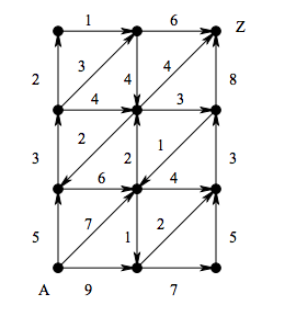
\includegraphics[width=.4\textwidth]{q72.png}
\end{center}
\end{figure}

Here we have a flow value of 8 and a cut of capacity 8. Thus by the Max Flow-Min Cut Theorem, this cut is a minimum cut and this flow value is a maximal flow.

\end{document} 